\documentclass[11pt,letterpaper,boxed]{hmcpset}
\usepackage{fullpage}
\setlength{\parskip}{6pt}
\setlength{\parindent}{0pt}
\usepackage[margin=1in]{geometry}
\usepackage{graphicx}
\usepackage{enumerate}
\usepackage{marvosym}
\usepackage{amssymb}
\usepackage{wasysym}
\usepackage{gensymb}
\usepackage{mathrsfs}
\usepackage{scrextend}
\usepackage{mathtools}
\usepackage{pgfplots}
\usepackage{xspace}
\usepackage[colorlinks]{hyperref}

\makeatletter
\renewcommand*\env@matrix[1][*\c@MaxMatrixCols c]{%
   \hskip -\arraycolsep
   \let\@ifnextchar\new@ifnextchar
   \array{#1}}
\makeatother

% --- style --- %
\renewcommand{\labelenumi}{{ (\alph{enumi})}}
\newcommand{\sand}{\quad \mbox{ and } \quad}
%\newcommand{\ds}{\displaystyle}
\allowdisplaybreaks

% --- making \xi look less awful --- %
\DeclareSymbolFont{CMletters}{OML}{cmm}{m}{it}
\DeclareMathSymbol{\xi}{\mathord}{CMletters}{"18}

% --- math --- %
\newcommand{\Z}{\mathbb{Z}}
\newcommand{\R}{\mathbb{R}}
\newcommand{\C}{\mathbb{C}}
\newcommand{\Q}{\mathbb{Q}}


\newcommand{\Lt}[1]{\mathcal{L}\crb{#1}}
\newcommand{\ilt}[1]{\mathcal{L}^{-1}\crb{#1}}

\newcommand{\pn}[1]{\left( #1 \right)}
\newcommand{\sqb}[1]{\left[ #1 \right]}
\newcommand{\crb}[1]{\left\{ #1 \right\}}
\newcommand{\lra}[1]{\left\langle #1 \right\rangle}
\newcommand{\magn}[1]{\left\lVert #1 \right\rVert}

\newcommand{\pdr}[2]{\frac{\partial #1}{\partial #2}}
\newcommand{\im}[1]{\text{im}\pn{#1}}
\newcommand{\m}[1]{\Z/#1\Z}

\newcommand{\VEC}[1]{\ensuremath{\mathbf{#1}}\xspace}
\DeclareMathOperator{\proj}{proj}
\newcommand{\vectorproj}[2][]{\proj_{\VEC{#1}}\VEC{#2}}

\newenvironment{amatrix}[1]{%
  \left(\begin{array}{@{}*{#1}{c}|c@{}}
}{%
  \end{array}\right)
}

\makeatletter
\renewcommand*\env@matrix[1][*\c@MaxMatrixCols c]{%
  \hskip -\arraycolsep
  \let\@ifnextchar\new@ifnextchar
  \array{#1}}
\makeatother

\newcommand{\spn}[1]{\text{span}\pn{#1}}

\newcommand*\Heq{\ensuremath{\overset{\kern2pt H}{=}}}

\name{Box \#$\rule{1cm}{0.15mm}$}
\class{Math 65 Section 1}
\assignment{Homework 9}
\duedate{30 May 2018}

\begin{document}

%\begin{center}
\noindent\textbf{Collaborators:} 
%\end{center} 



\begin{problem}[1.] ({\bf The Lorenz Equations}) Consider the  nonlinear system
\begin{eqnarray*}
x' & = & \sigma ( y - x) \\
y' & = & r x - y - x z \\
z'  & = & -\beta z + x y
\end{eqnarray*}
where $\sigma,  r,$ and $\beta$ are positive constants. To simplify, let $\beta=1$ and $\sigma=3$ throughout.

\begin{enumerate}
\item[(a)] By inspection, there is an equilibrium point at the origin $(0,0,0)$.  Show that the 
origin is {\it asymptotically stable} for $0<r<1$ and {\it unstable} for $r>1$. 
\item[(b)]Show that for $r>1$ the system has three equilibrium points. \end{enumerate}
\end{problem}

\begin{solution}
\vfill
\end{solution}
\newpage

\begin{problem}[2.]  Consider the nonlinear  system
\begin{eqnarray*}
\dot{x} & =& y-x \\
\dot{y} &=& 2xy-2y 
\end{eqnarray*}
\begin{itemize}
\item[(a)] Find all equilibrium points of the system. 
\item[(b)] Compute the Jacobian matrix $D\mathbf{f}$ at each equilibrium point, and find the associated eigenvalues and eigenvectors for the linearization. 
\item[(c)]  Assuming the linearization is accurate use your information from part (b) to sketch the phase portrait near each equilibrium point. You don't need to draw the entire phase portrait, just what your linear models predict the system looks like near the equilibrium points.   Classify each equilibrium point by type (e.g., nodal sink, nodal source, spiral sink, spiral source, center, saddle, degenerate node) and stability (e.g., stable, asymptotically stable, or unstable).
\end{itemize}
\end{problem}


\begin{solution}
\vfill
\end{solution}
\newpage


\begin{problem}[3.]
Consider a  population model for rabbits, $x(t) \geq 0$, and  hares, $y(t) \geq 0$
(measured in arbitrary units, chosen to make the math nicer):  
\begin{eqnarray*}
\dot{x} & =& x (4 - x - 3y) \cr
\dot{y} &=& y (4- 3x -y) 
\end{eqnarray*}
\noindent
\parbox{0.5\textwidth}{
\[ 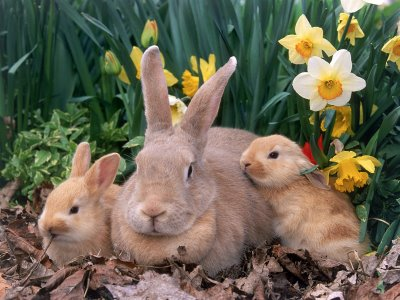
\includegraphics[width=0.33\textwidth]{rabbits.jpg}  \]
\[  x(t) \]
}
\parbox{0.5\textwidth}{
\[ 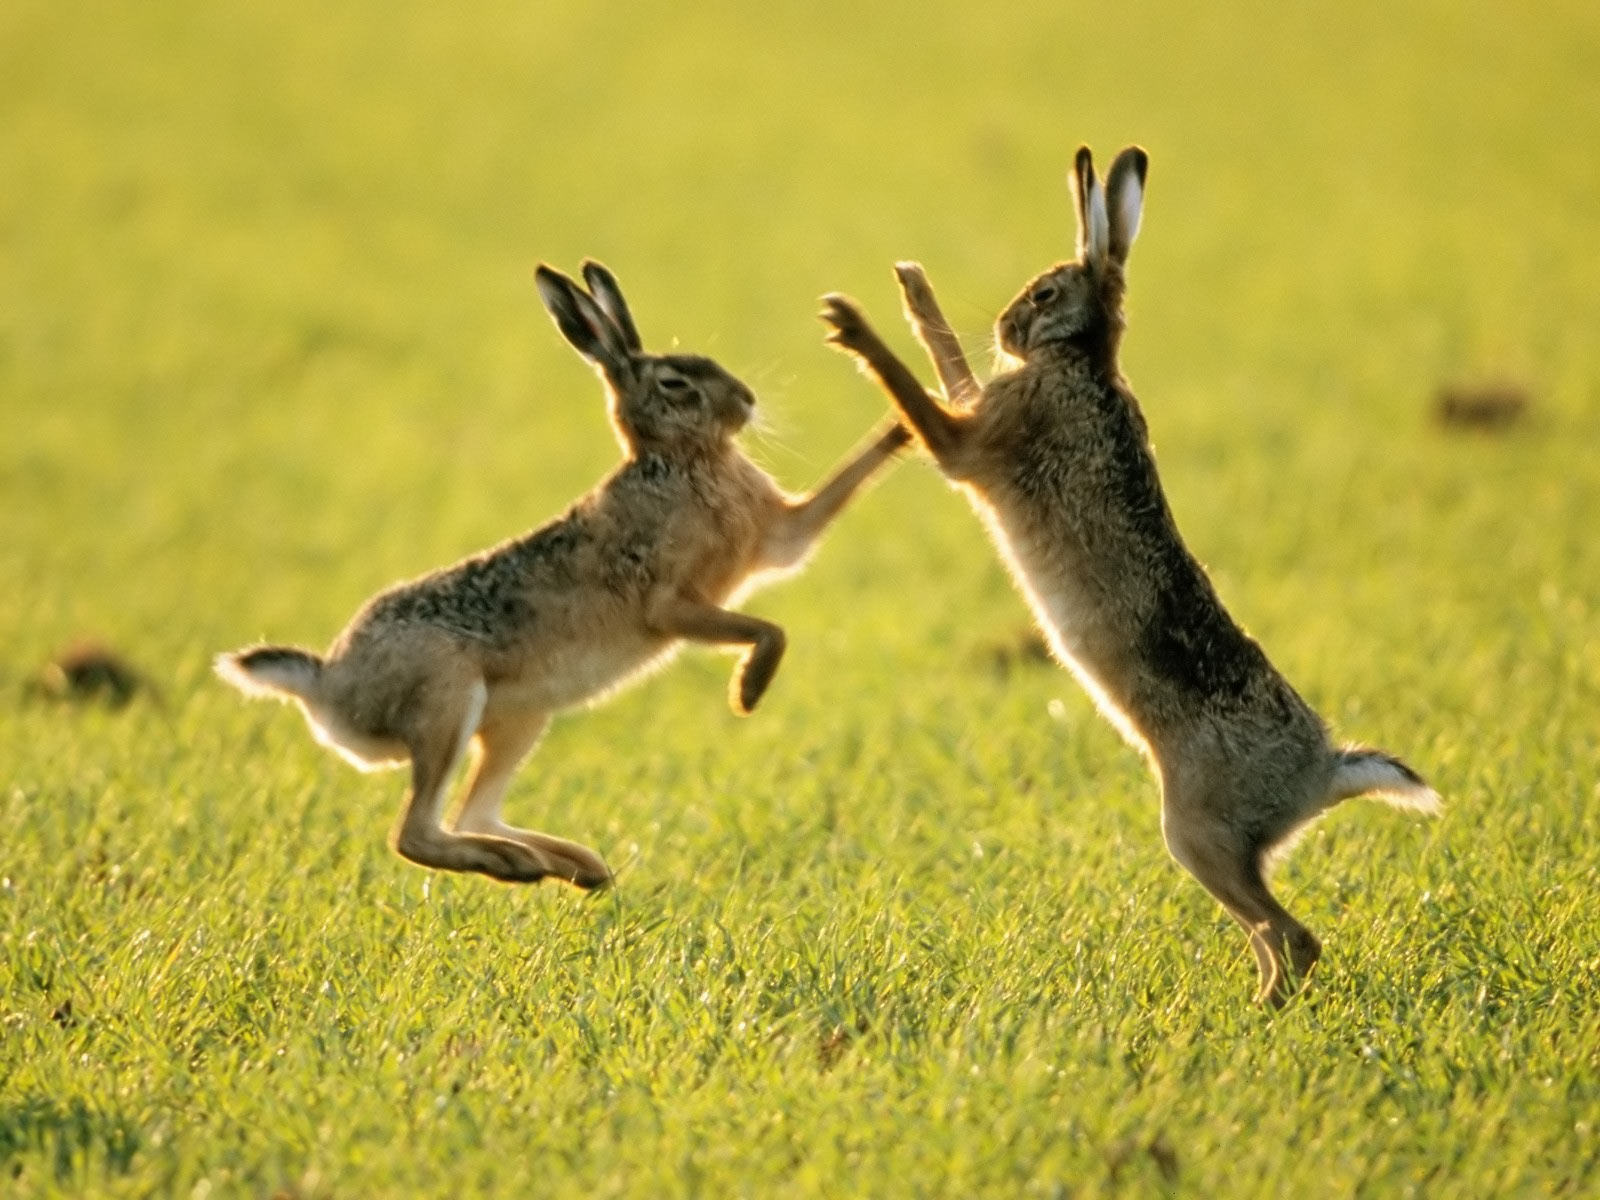
\includegraphics[width=0.33\textwidth]{hares.jpg}  \]
\[  y(t) \]
}

\begin{enumerate}
\item[(a)] Determine all equilibrium points of the system.
\item[(b)]
Linearize the system at each equilibrium
point,  and find the eigenvalues and eigenvectors of the resulting linear system. 
Classify each equilibrium point
by type  and stability.

\item[(c)] Assuming the linearization is accurate, 
use your results from (b) to sketch the phase portrait (you can check with pplane or other software to help connect your local linear information more globally). Recall $x,y
\geq 0$, so you only need to plot the orbits in the first quadrant. Note: don't skimp on the real estate, draw a healthy size first quadrant so you can clearly indicate the various details.
 \item[(d)] (principle of competitive exclusion)
 Assuming that we start with a nonzero population of rabbits
and hares, what does the model predict for the populations at large time?  
\end{enumerate}
\end{problem}


\begin{solution}
\vfill
\end{solution}
\newpage


\begin{problem}[4.]  We return to  the SIR Model 
\begin{eqnarray}
\label{s2} \nonumber
\dot{S}& = & -\alpha S I \\
\label{i2} \nonumber
\dot{I} & = & \alpha S I - \beta I \\
\dot{R} & = & \beta I,  \nonumber
\end{eqnarray}
where $\alpha, \beta > 0$.  The state variables  $S$ and $I$  form a closed subsystem, so to analyze the SIR model it is sufficient to study the two-dimensional system
\begin{eqnarray}
\label{s}
\dot{S} & = & -\alpha S I \\
\label{i}
\dot{I} & = & \alpha S I - \beta I 
\end{eqnarray}
We are only concerned with the dynamics  in the first quadrant ($S \geq 0, I \geq 0$). 
\begin{enumerate}
\item[(a)] In the previous assignment we found any point of the form $(S_0,0)$ is an equilibrium point. Show that the linearization at any such point has $0$ as an eigenvalue.  Show that the other eigenvalue is positive when $S_0 > \frac{\beta}{\alpha}$ and negative when $S_0 < \frac{\beta}{\alpha}$.  
\item[(b)] Let $\beta =1$ and $\alpha = 2$. Use pplane (or some other software) to plot some sample  phase portraits  assuming $0 \leq S \leq 1$. Choose your axes to ensure all the key behavior of the model is demonstrated in your figure. 
\item[(c)] If we start near the disease free equilibrium state $(1,0)$ (e.g., if the initial state is $(0.999,0.001)$, modeling the introduction of the disease into a population that is all susceptible), what does the model predict for the values of $S(t)$ and $I(t)$ as $t \to \infty$? 
\end{enumerate}

\noindent
\parbox{0.5\textwidth}{
\[ 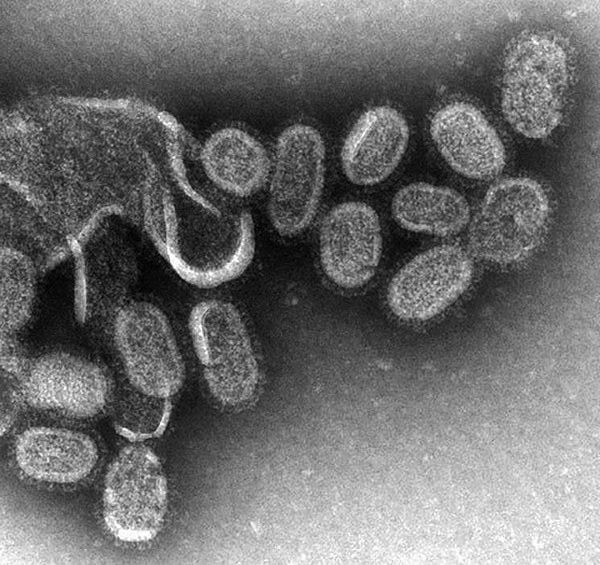
\includegraphics[width=0.41\textwidth]{em-flu.jpg}  \]
\[  \text{influenza virions} \]
}
\parbox{0.5\textwidth}{
\[ 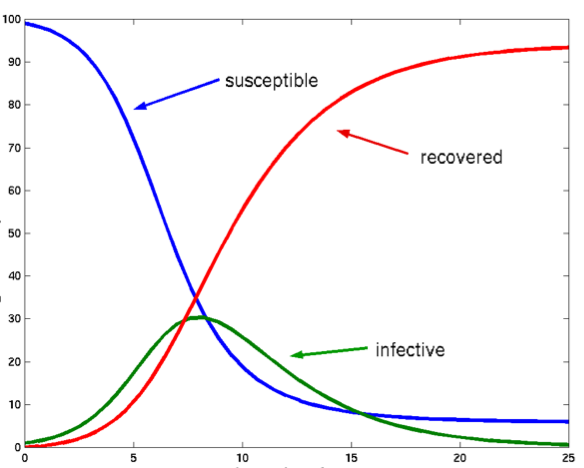
\includegraphics[width=0.5\textwidth]{sir.png} \]
\[  \text{sample time series of $S(t),I(t),R(t)$} \]
}
\end{problem}

\begin{solution}
\vfill
\end{solution}
\newpage

\end{document}







